
\pagebreak

\section*{Introduction}
\addcontentsline{toc}{section}{Introduction}
%\markboth{Introduction}{} 
Comme TV5 monde en 2015, les pertes des entreprises victimes de cyberattaques se comptent souvent en dizaines de millions d'euros. L'Open Web Application Security Project (OWASP : {\color{blue} \url{https://www.owasp.org}}), publie régulièrement la liste des 10 menaces les plus critiques qui concernent les applications web. Une manière de s'en prémunir consiste à pratiquer le hacking web éthique. C'est là qu'entre en scène l'outil DVWA. Damn Vulnerable Web App ({\color{blue} \url{http://www.dvwa.co.uk}}), est un environnement PHP qui permet de se former à la sécurité des sites web. Le hacker en herbe peut ainsi se former et tester légalement ses compétences sur une application hébergée en local. 

\begin{figure}[!h]
	\begin{center}
		\label{10_menaces}
		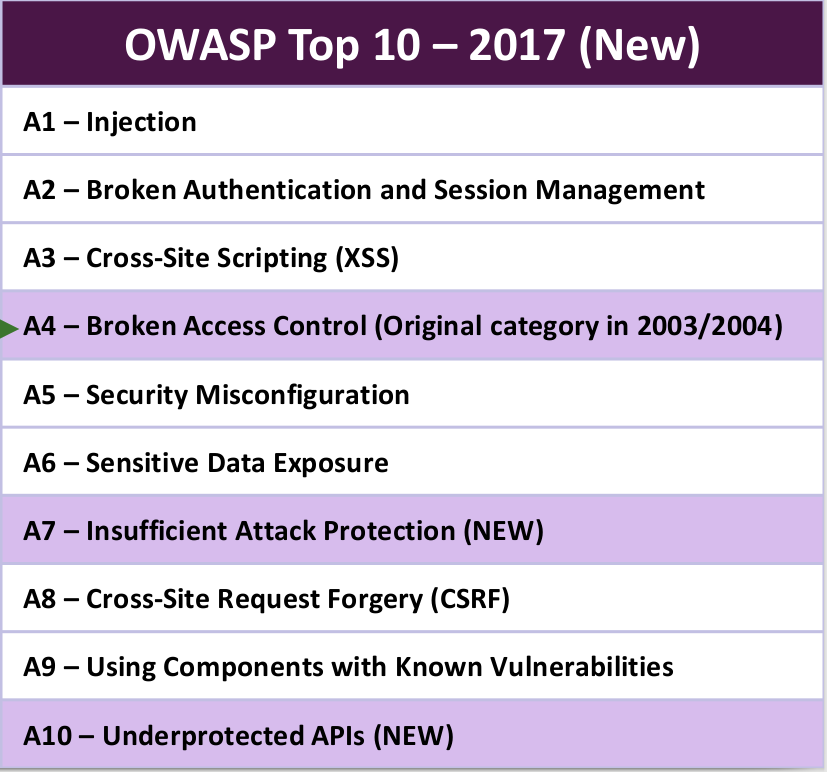
\includegraphics[scale=0.4]{images/10_menaces.png}
		\caption{Le top 10 des menaces web 2017 publiées par l'OWASP}
	\end{center}
\end{figure}

\section{Installation de la plateforme de test}
Une solution possible consiste à installer la distribution kali et le site web DVWA sur une machine virtuelle virtualBox.
Il suffit ensuite de modifier la configuration réseau NAT de la machine virtuelle en accès par pont.
La commande hostname -I sur la machine virtuelle fournit son adresse IP, par exemple 192.168.1.8. Il ne reste plus qu'à se connecter via firefox
au site dvwa via {\color{blue}http://192.168.1.8/dvwa/}. Le login par défaut est admin/password.

 \begin{figure}[!h]
 	\begin{center}
 		\label{}
 		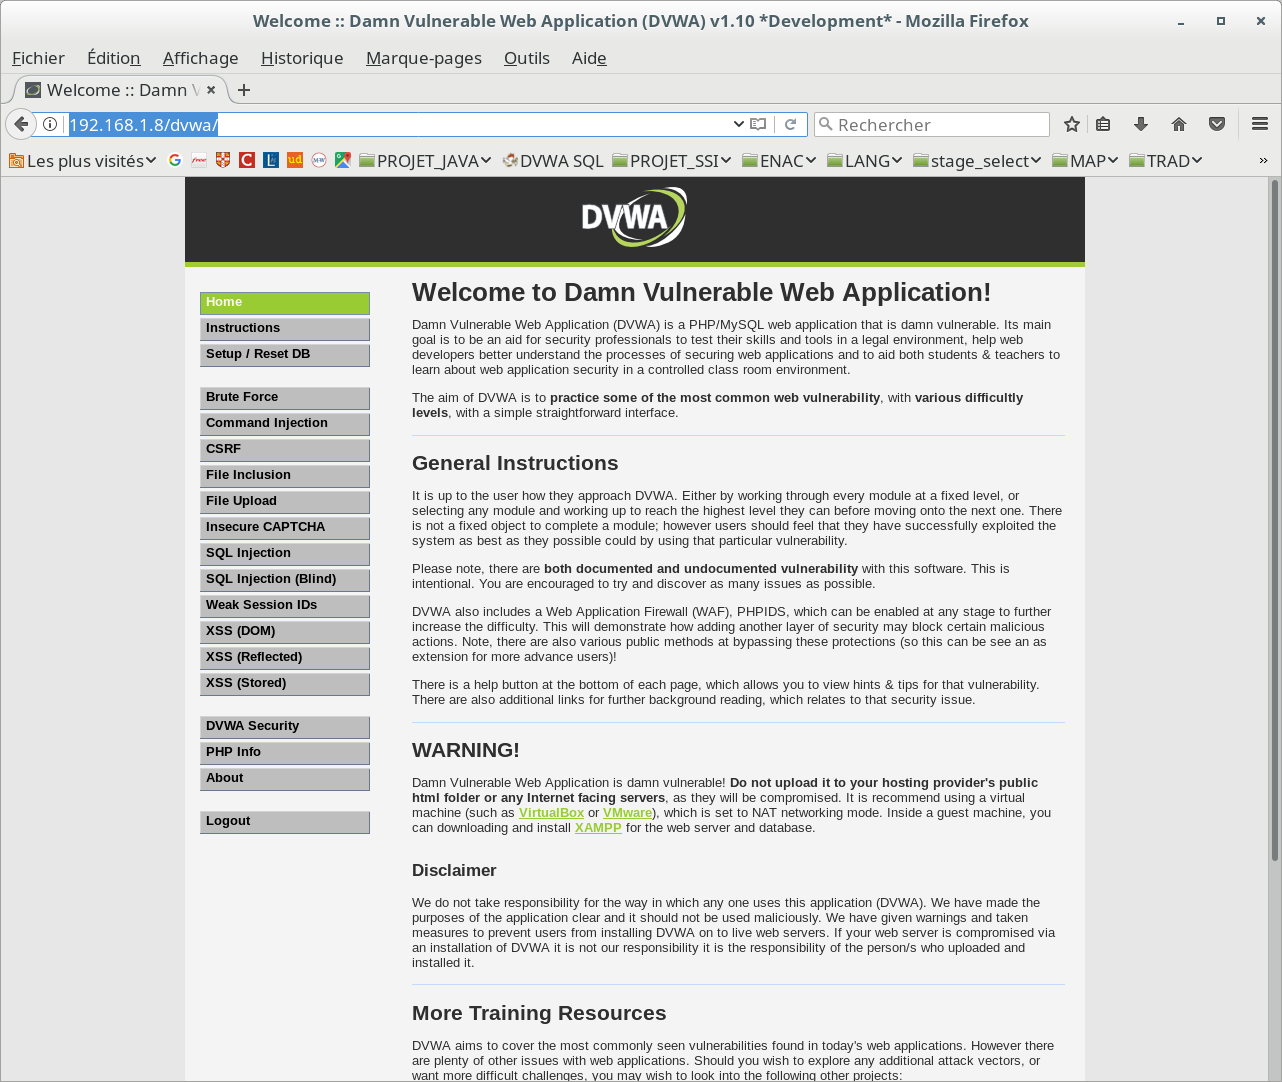
\includegraphics[scale=\scaledvwa]{images/dvwa.png}
 		\caption{Accès à DVWA à partir du navigateur de la machine hôte. Le site web DVWA est installé sur une machine virtuelle kali linux.}
 	\end{center}
 \end{figure}


